\chapter{Introduction}
\section{Introduction}
General relativity is the theory of space, time, and gravitation formulated by Einstein in 1915. It is often regarded as a very abstruse and difficult theory, partly because the new viewpoint it introduced on the nature of space and time takes some effort to get used to since it goes against some deeply ingrained, intuitive notions, and partly because the mathematics required for a precise formulation of the ideas and equations of general relativity (namely, differential geometry) is not familiar to most physicists. Although it has been universally acknowledged as being a beautiful theory, the potential relevance of general relativity to the rest of physics has not been universally acknowledged and, indeed, probably for this reason, the subject has lain nearly dormant during much of its history.

Strong interest in general relativity began to be revived starting in the late 1950s, particularly by the Princeton group led by John Wheeler and the London group led by Herman Bondi. Although it is difficult to determine the reasons for trends in physics, two developments-relating general relativity to other areas of physics and astronomy-have contributed greatly to the sustained interest in general relativity which has continued since then. The first is the astronomical discovery of highly energetic, compact objects-in particular, quasars and compact X-ray sources. It is likely that gravitational collapse and/or strong gravitational fields play an important role here, and if so, general relativity would be needed to understand the structure of these objects. The modern theory of gravitational collapse, singularities, and black holes was developed beginning in the mid-1960s largely in response to this impetus. 

A second factor promoting renewed interest in general relativity is the realization that although gravitation may be too weak to play an important role in laboratory experiments in particle physics, nevertheless it is of great importance to our further understanding of the laws of nature that a quantum theory of gravitation be developed. In order to make progress toward this goal, a deeper understanding of some aspects of the classical theory of gravitation-general relativity-may be needed. Interest in this program has been greatly strengthened by the prediction of quantum particle creation in the gravitational field of a black hole, as well as by advances in the study of gauge theories in particle physics.

But even aside from the potential impact of general relativity on astronomy and on other branches of physics, the theory in its own right makes many remarkable statements concerning the structure of space and time and the nature of the gravitational field. After one has learned the theory, one cannot help feeling that one has gained some deep insights into how nature works.

The purpose of this book is to present the theory of general relativity. We will take a more modem, geometrical viewpoint than Einstein had, and we will, of course, discuss the recent advances and developments, but the essential content of the theory is the one Einstein gave over half a century ago. We begin in this chapter by discussing the structure of space and time and the basic ideas of relativity theory from an intuitive, physical point of view. More complete introductory discussions are given by Geroch (1978a) and Wald (1977a). The remainder of this book will be devoted to making these ideas mathematically precise and exploring their consequences.

\section{Space and Time in Prerelativity Physics and in Special Relativity}

Perhaps the greatest obstacle to understanding the theories of special and general relativity arises from the difficulty in realizing that a number of previously held basic assumptions about the nature of space and time are simply wrong. We begin, therefore, by spelling out some key assumptions about space and time. In both the past and modern viewpoints, space and time have at least the following structure in common. We can consider space and time (≡ spacetime) to be a continuum composed of \emph{events}, where each event can be thought of as a point of space at an instant of time. Furthermore, all events (or, at least, all events in a sufficiently small neighborhood of a given event) can be uniquely characterized by four numbers: in ordinary language, three numbers for the spatial position and one for the time. As will be discussed in chapter 2, a mathematically precise statement of these ideas is that spacetime is a four-dimensional manifold.

However, prior to relativity theory it was believed that spacetime had the following additional structure: Given an event $p$ in spacetime, there is a natural, observer-independent notion of events occurring ``at the same time'' as $p$. More precisely, given two events $p$ and $q$, one of the following three mutually exclusive possibilities must hold
\begin{enumerate}[label=(\arabic*)]
    \item It is possible, in principle, for an observer or material body to go from event $q$ to event $p$, in which case one says $q$ is to the past of $p$.
    \item It is possible to go from $p$ to $q$, in which case one says $q$ is to the future of $p$.
    \item It is impossible, in principle, for an observer or material body to be present at both events $p$ and $q$.
\end{enumerate}

\begin{figure}[!ht]
\begin{minipage}{.6\textwidth}
    \centering
    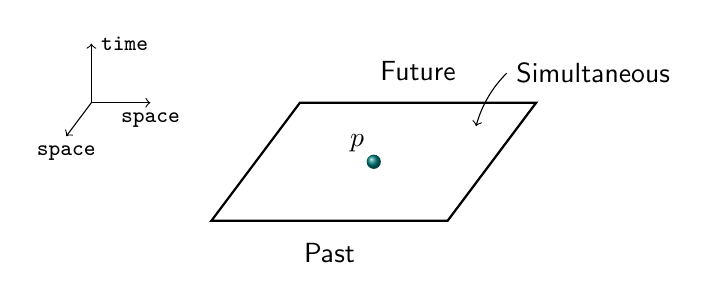
\begin{tikzpicture}[scale=1.5]
        \draw [->, xshift=-.4in] (0,1) -- (.5,1) node [anchor=north] {\ttfamily\footnotesize space};
        \draw [->, xshift=-.4in] (0,1) -- (0,1.5) node [anchor=west] {\ttfamily\footnotesize time};
        \draw [->, xshift=-.4in] (0,1) -- ({-.3/sqrt(2)},{1-.4/sqrt(2)}) node [anchor=north] {\ttfamily\footnotesize space};
        \draw [thick] (0,0) -- (2,0) node [midway,anchor=north, yshift=-1ex] {\sffamily Past} -- (2.75,1) -- (.75,1) node [midway,anchor=south, yshift=1ex] {\sffamily Future} -- cycle;
        \shade [ball color=teal] (1.375,.5) circle (.06) node [anchor=south east] {$p$};
        \draw [->] (2.5,1.25) arc (135:165:1) node [anchor=west,at start] {\sffamily Simultaneous};
    \end{tikzpicture}
\end{minipage}
\hfill
\begin{minipage}{.32\textwidth}
    \caption{A diagram showing the causal structure of spacetime in prerelativity physics. Given an event $p$, all other events in spacetime either are to the future of $p$, to the past of $p$, or Simultaneous with $p$. The simultaneous events form a three-dimensional surface in spacetime.}
    \label{1.1}
\end{minipage}
\end{figure}

In prerelativity physics, events in the third category are assumed to form a three-dimensional set and define the notion of simultaneity with $p$, as is illustrated in \figref{1.1}.

The belief that the causal structure of spacetime has the character shown in \figref{1.1} turns out to be wrong. In special relativity theory the above classification of the causal relationships between events still holds. The crucial difference is that events in category (3) form more than a three-dimensional set; the causal relation between $p$ and other events has the structure sketched in \figref{1.2}. The events in category (3) can be further subdivided as follows
\begin{itemize}
    \item Events that lie on the boundary of the set of points to the future of $p$. These events cannot be reached by a material particle starting at $p$ but can be reached by a light signal emitted from p. They form the ``future light cone'' of $p$ (a three-dimensional set).
    \item Events on the past light cone of $p$, defined similarly.
    \item Events in category (3) which are on neither the past nor the future light cone. These events are said to be spacelike related to $p$ and comprise a four-dimensional set.
\end{itemize}
    
A key fact closely related to the above is that in special relativity there is no notion of absolute simultaneity; there are no absolute three-dimensional surfaces in space-time as in \figref{1.1}. As we shall see below, an observer still can define a notion of which events occur ``at the same time'' as a given event-thus defining a three-dimensional surface in spacetime—but the notion he gets depends upon his state of motion. (On the other hand, the light cones of \figref{1.2} \emph{are} absolute surfaces.) The notion that there is absolute simultaneity is a deeply ingrained one. The fact that there is no such notion is one of the most difficult ideas to adjust to in the theory of special relativity.

\begin{figure}[!ht]
\begin{minipage}{.32\textwidth}
    \caption{A diagram showing the causal structure of spacetime in special relativity. The ``light cone'' of $p$ rather than a ``surface of simultaneity'' with $p$ now plays a fundamental role in determining the causal relationship of $p$ to other events.}
    \label{1.2}
\end{minipage}
\hfill
\begin{minipage}{.64\textwidth}
    \centering
    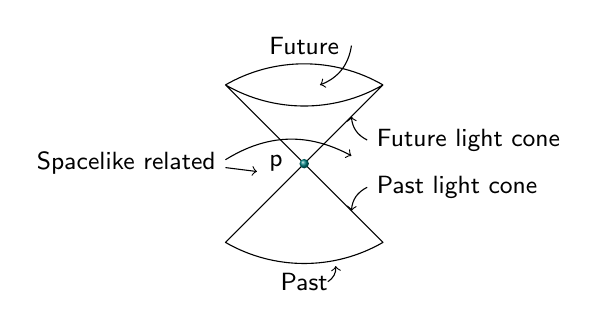
\begin{tikzpicture}
        \draw [line join=round,line cap=round] (-1,1) -- (1,-1) arc (-60:-120:2) -- (1,1) arc (-60:-120:2) arc (-60:-120:-2);
        \shade [ball color=teal] (0,0) circle (.06) node [anchor=east,xshift=-1ex] {\sffamily\small p};
        \node at (0,1.5) {\sffamily\small Future};
        \path [->] (.6,1.5) edge [bend left] (.2,1);
        \node at (0,-1.5) {\sffamily\small Past};
        \path [->] (.3,-1.5) edge [bend right] (.4,-1.3);
        \node [left] at (-1,0) {\sffamily\small Spacelike related};
        \path [->] (-1,-.05) edge (-.6,-.1);
        \path [->] (-1,.05) edge [bend left] (.6,.1);
        \node [right] at (.8,.3) {\sffamily\small Future light cone};
        \path [->] (.8,.3) edge [bend left] (.6,.6);
        \node [right] at (.8,-.3) {\sffamily\small Past light cone};
        \path [->] (.8,-.3) edge [bend right] (.6,-.6);
    \end{tikzpicture}
\end{minipage}
\end{figure}

In special relativity (as in prerelativity physics) one has the notion of inertial, ``nonaccelerating'' motion, namely the motion a material body would undergo if subjected to no external forces. An inertial observer can label the events of spacetime in the following manner. He can build himself a rigid frame and label the grid points of the frame with the Cartesian coordinates $x, y, z$ of the (assumed Euclidean) geometry of the frame. He can then have a clock placed at each grid point and can synchronize each clock with his by a symmetrical procedure, e.g., by making sure that a given clock and his give the same reading when they receive a signal sent out in a symmetrical manner by an observer stationed halfway between the two. (Because the causal structure of spacetime is that of \figref{1.2}, not \figref{1.1}, synchronization is not a trivial issue.) The observer may carry the grid, complete with synchronized clocks, in a nonrotating manner. Each event in spacetime can now be labeled with the coordinates $x, y, z$ of the grid point at which the event occurred and the reading $t$ of the (synchronized) clock at that event. The labels $t, x, y, z$ assigned to events in this manner are referred to as global inertial coordinates. 

If two such inertial observers go through this procedure, one may compare the coordinate labels they assign to events. In prerelativity physics (where the same labeling procedure works, the only difference being that clock synchronization \emph{is} trivial), if observer $O$ labels an event $p$ with coordinates $t, x, y, z$ and $O'$ moves with velocity $\vv{v}$ in the $x$-direction, passing observer $O$ at the event labeled $t = x = y = z = 0$. the coordinate labels that $O'$ assigns to event $p$ are

\begin{align}
    & t'=t\label{1.2.1}\\
    & x'=x-vt\label{1.2.2}\\
    & y'=y\label{1.2.3}\\
    & z'=z\label{1.2.4}
\end{align}

In special relativity, however, the labeling by $O'$ will be related that of $O$ by a Lorentz transformation
\begin{align}
    & t'=(t-vx/c^2)/(1-v^2/c^2)^{1/2}\label{1.2.5}\\
    & x'=(x-vt)/(1-v^2/c^2)^{1/2}\label{1.2.6}\\
    & y'=y\label{1.2.7}\\
    & z'=z\label{1.2.8}
\end{align}

where $c$ is the speed of light. \eqref{1.2.5} shows that the notion of simultaneity determined by $O$ (namely, $t = \text{constant}$) differs from that determined by $O'$ ($t' = \text{constant}$), as illustrated in \figref{1.3}.

\begin{figure}[!ht]
    \centering
    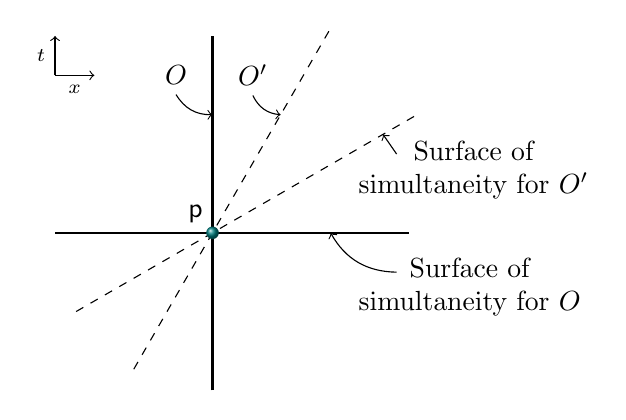
\begin{tikzpicture}
        \draw [->, xshift=-2 cm,yshift=2 cm] (0,0) -- (.5,0) node [anchor=north,midway] {$\scriptstyle x$};
        \draw [->, xshift=-2 cm, yshift=2 cm] (0,0) -- (0,.5) node [anchor=east,midway] {$\scriptstyle t$};
        \draw [thick] (-2,0) -- (2.5,0);
        \draw [thick] (0,-2) -- (0,2.5);
        \draw [dashed] ({-sqrt(3)},-1) -- ({3*sqrt(3)/2},1.5);
        \draw [dashed] (-1,{-sqrt(3)}) -- (1.5,{3*sqrt(3)/2});
        \shade [ball color=teal] (0,0) circle (.08) node [anchor=south east] {\sffamily p};
        \node [align = center,right] at ({sqrt(3)},.8) {Surface of\\simultaneity for $O'$};
        \draw [->] ({1.35*sqrt(3)},1) -- ({5*sqrt(3)/4},1.25);
        \node [align = center,below right] at ({sqrt(3)},-.2) {Surface of\\simultaneity for $O$};
        \path [->] ({1.35*sqrt(3)},-.5) edge [bend left] (1.5,0);
        \node [left] (O) at (-.2,2) {$O$};
        \path [->] (O.south) edge [bend right] (0,1.5);
        \node [right] (O') at (.2,2) {$O'$};
        \path [->] (O'.south) edge [bend right] ({sqrt(3)/2},1.5);
    \end{tikzpicture}
    \caption{A spacetime diagram illustrating the fact that in special relativity the inertial observers $O$ and $O'$ disagree over the definition of simultaneity with event $p$.}
    \label{1.3}
\end{figure}

\section{The Spacetime Metric}

In the previous section, we gave a prescription for how an inertial observer $O$ can label the events in spacetime with global inertial coordinates $t, x, y, z$. However, a fundamental tenet of special relativity is that there are no preferred inertial observers. As seen above. a different inertial observer using the same procedure assigns different labels $t',x',y',z'$ to the events in spacetime. Thus, the coordinate labels themselves do not have intrinsic significance since they depend as much on which observe does the labeling as they do on the properties of spacetime itself. It is of great interest to determine what quantities have absolute, observe-independent significance, i.e., truly measure intrinsic structure of spacetime. This is equivalent to determining what functions of global inertial coordinates are independent of the choice of inertial frame.

In prerelativity physics the answer is the following. The time interval $\Delta t$ between two events has absolute significance; all observers will agree on the value of $\Delta t$. Furthermore, the spatial interval $\abs{\Delta\vv{x}}$ between two simultaneous events is observer independent. However, these quantities (or functions of them) are the only ones with absolute significance. For example, observers moving with nonzero relative velocity will disagree over the spatial interval between nonsimultaneous events. In special relativity neither the time interval nor the space interval between ``relatively simultaneous'' events (i.e., events determined to be simultaneous by a particular observer) has absolute significance. The quantity which is observer independent is the spacetime interval, $I$, defined by
\begin{equation}
    I=-(\Delta t)^2+\frac{1}{c^2}\ab[(\Delta x)^2+(\Delta y)^2+(\Delta z)^2]
    \label{1.3.1}
\end{equation}

Indeed, the Poincaré transformations (the set of all possible transformations between global inertial coordinates) consist precisely of the linear transformations which leave $I$ unchanged. The spacetime interval $I$ and functions of $I$ are the only observer-independent quantities characterizing the spacetime relationships between events.

What is truly remarkable about the expression for $I$ is that it is quadratic in the coordinate differences, just like the distance function in Euclidean (i.e., flat, positive definite) geometry. Indeed, the only difference is the minus sign in front of $(\Delta t)^2$, allowing $I$ to become zero or negative. We shall refer to $I$ as the metric of spacetime in analogy to an ordinary Euclidean metric. (More precisely, the metric of spacetime in special relativity will be defined later to be a tensor field associated with the formula for the spacetime interval between two ``infinitesimally nearby'' events; see \eqref{4.2.2} below.) As we shall see in chapter 3, this difference in metric signature makes very little difference in the mathematical analysis of metrics. In particular definitions of geodesics (``straightest possible lines'') and curvature carry through in the same way for metrics with the signature of $I$ as for ordinary positive definite metrics. It is interesting to note that, as discussed more fully in chapter 4, the paths in spacetime of inertial observers in special relativity are geodesics of the spacetime metric, and the curvature associated with $I$ is zero, i.e., the spacetime geometry in special relativity is flat.

\section{General Relativity}
Prior to special relativity, the prerelativity notions of space and time pervaded-among many other things-the formulation of the laws of physics. When these notions were overthrown, the task remained of modifying and reformulating physical laws to be consistent with the spacetime structure given by the theory of special relativity. Maxwell's theory of electromagnetism was already consistent with special relativity. Indeed, its incompatibility with prerelativity notions of spacetime structure unless preferred inertial frames were introduced led directly to the discovery of special relativity. Newton's theory of gravitation is not consistent with special relativity since it invokes notions of instantaneous influence of one body on another, but it might be thought that one could simply modify it to fit within the framework of special relativity.

However, two key ideas motivated Einstein \emph{not} to follow this path but rather to seek an entirely new theory of spacetime and gravitation-a theory that revolutionized our notions of space and time every bit as much as special relativity already had done.

The first idea is that \emph{all} bodies are influenced by gravity and, indeed, all bodies fall precisely the same way in a gravitational field. This fact, known as the \emph{equivalence principle}, is expressed in the Newtonian theory of gravitation by the statement that the gravitational force on a body is proportional to its inertial mass. Because motion is independent of the nature of the bodies, the paths of freely falling bodies define a preferred set of curves in spacetime just as in special relativity the paths in spacetime of inertial bodies define a preferred set of curves, independent of the nature of the bodies. This suggests the possibility of ascribing properties of the gravitational field to the structure of spacetime itself. As already mentioned in the previous section, the paths of inertial bodies in special relativity are geodesics of the spacetime metric. Perhaps, then, the paths of freely falling bodies are always geodesics, but the spacetime metric is not always that given by special relativity. What we think of as a gravitational field would then not be a new field at all, but rather would correspond to a deviation of the spacetime geometry from the flat geometry of special relativity. We shall discuss these ideas further in chapter 4.

The second much less precise set of ideas which motivated the formulation of general relativity goes under the name of \emph{Mach's principle}. In special relativity as in prerelativity notions of spacetime, the structure of spacetime is given once and for all and is unaffected by the material bodies that may be present. In particular, ``inertial motion'' and ``nonrotating'' are not influenced by matter in the universe. Mach as well as a number of earlier philosophers and scholars (in particular, Riemann) found this idea unsatisfactory. Rather, Mach felt that all matter in the universe should contribute to the local definition of ``nonaccelerating'' and ``nonrotating''; that in a universe devoid of matter there should be no meaning to these concepts. Einstein accepted this idea and was strongly motivated to seek a theory where, unlike special relativity, the structure of spacetime is influenced by the presence of matter.

The new theory of space, time, and gravitation-general relativity-proposed by Einstein states the following: The intrinsic, observer-independent, properties of spacetime are described by a spacetime metric, as in special relativity. However, the spacetime metric need not have the (flat) form it has in special relativity. Indeed, curvature, i.e., the deviation of the spacetime metric from flatness, accounts for the physical effects usually ascribed to a gravitational field. Furthermore, the curvature of spacetime is related to the stress-energy-momentum tensor of the matter in spacetime via an equation postulated by Einstein. In this way, the structure of spacetime (as embodied in the spacetime metric) is related to the matter content of spacetime, in accordance with some (but not all!) of Mach's ideas. Thus far, the predictions of general relativity have been found to be in excellent agreement with experiments and observations (see section 6.3 below and Will 1981).

Most of the remainder of this book is devoted to exploring the consequences of this theory. Our first task, however, is to give a precise, mathematical expression to the ideas discussed in this chapter. To begin with, we must give a precise formulation of the notion that spacetime is a four-dimensional continuum. This will be accomplished with the definition of a manifold given in section 2.1. We must then introduce the basic mathematical framework needed to discuss curved geometry: vectors and tensors (2.2), the metric (2.3), derivative operators (3.1), curvature (3.2), and geodesics (3.3). Almost all of the discussion we shall give applies equally well to the differential geometry of ordinary surfaces (positive definite metric) as to the geometry of spacetime (metric of Lorentz signature). After development of these mathematical tools and techniques, we will then be in position to begin our study of general relativity in chapter 4.

\begin{problem}
    \emph{Car and garage paradox}: The lack of a notion of absolute simultaneity in special relativity leads to many supposed paradoxes. One of the most famous of these involves a car and a garage of equal proper length. The driver speeds toward the garage, and a doorman at the garage is instructed to slam the door shut as soon as the back end of the car enters the garage. According to the doorman, ``the car Lorentz contracted and easily fitted into the garage when I slammed the door.'' According to the driver, ``the garage Lorentz contracted and was too small for the car when I entered the garage.'' Draw a spacetime diagram showing the above events and explain what really happens. Is the doorman's statement correct? Is the driver's statement correct? For definiteness, assume that the car crashes through the back wall of the garage without stopping or slowing down.
\end{problem}

\begin{solution}

Let $c=1$. The spacetime diagram can be found below. In it the primed coordinates are those assigned to events by the driver and the unprimed ones are those assigned by the doorman. At the origin is the event ``the driver has just reached the doorman and is about to enter the garage''. It follows that the world lines of the driver and doorman are the $t'$-axis and the $t$-axis, respectively.

Let $L$ denote the common proper length of the car and the garage. The world line of the back wall of the garage is thus the one parallel to the $t$-axis and passing through the point $(x,t)=(L,0)$. Similarly, the world line of the rear end of the car is the one parallels to the $t'$-axis and passing through $(x',t')=(-L,0)$.

\columnratio{.32}
\begin{paracol}{2}
    \begin{center}
    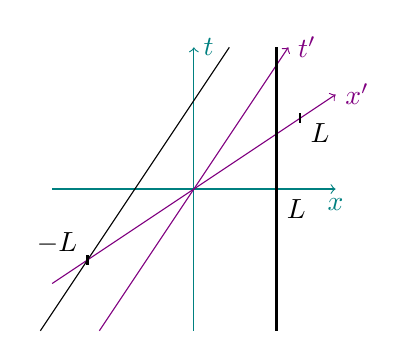
\begin{tikzpicture}[scale=.6]
        \draw [->,teal] (-3,0) -- (3,0) node [below] {$x$};
        \draw [->,teal] (0,-3) -- (0,3) node [right] {$t$};
        \draw [->,violet] (-2,-3) -- (2,3) node [right] {$t'$} ;
        \draw [->,violet] (-3,-2) -- (3,2) node [right] {$x'$} ;
    
        \draw [xshift=-1.25 cm] (-2,-3) -- (2,3);
        \draw [thick] (-2.25,-1.4) -- (-2.25,-1.6) node [above left] {$-L$};
        \draw [thick] (2.25,1.4) -- (2.25,1.6) node [below right] {$L$};
    
        \draw [thick] (1.75,3) -- (1.75,-3) node [midway, below right] {$L$};
    \end{tikzpicture}
    \end{center}
    \switchcolumn
    Analyzing the spacetime diagram, one concludes that both statements are correct.

    The intersection of the $t' = 0$ line with the world line of the back wall of the garage is at a smaller value of $x'$ than $L$. This agrees with the driver's account.
        
    Let $t_\text{slam}$ be time coordinate recorded by the doorman as he slams the door shut. This event is at the intersection of the world lines of the doorman and that of the car's rear end. The line $t = t_\text{slam}$ intersects the world line of the driver at a smaller value of $x$ than that of the back wall of the garage. This agrees with the doorman's statement.
\end{paracol}

So what happens here? The driver is correct to say he had crashed through the back wall of the garage by the time the doorman shuts the door. The doorman is also correct when he says the back wall was intact by the time he closed the door. This seems to be a contradiction since from both statements one would conclude that the car would and would have not crashed by the time the door was closed. It turns out this conclusion would be wrong. This is because the expression ``by the time the door was closed'' means different things to the driver and the doorman. To the driver, it refers to a line parallel to the $x'$-axis. To the doorman, the expression refers to those events in a line parallel to the $x$-axis.
\end{solution}